\documentclass{beamer}

\usecolortheme[light]{solarized}

\beamertemplatenavigationsymbolsempty

\usepackage{hyperref}
\usepackage{minted}

\usepackage{graphicx}
\usepackage{tikz}

\usetikzlibrary{calc, patterns}

\begin{document}

    \begin{frame}
        \begin{center}
            \Large

            ``I will not lecture you.''

            \normalsize
            \vspace{1cm}
            Vince\\
            \href{https://twitter.com/drvinceknight}{@drvinceknight}\\
            \texttt{knightva@cardiff.ac.uk}
        \end{center}


    \end{frame}

    \begin{frame}
        \begin{center}
            \textbf{Active learning increases student performance in
            science, engineering, and mathematics} Freeman et al. 2014 (PNAS)
        \end{center}
    \end{frame}

    \begin{frame}
        \begin{center}
            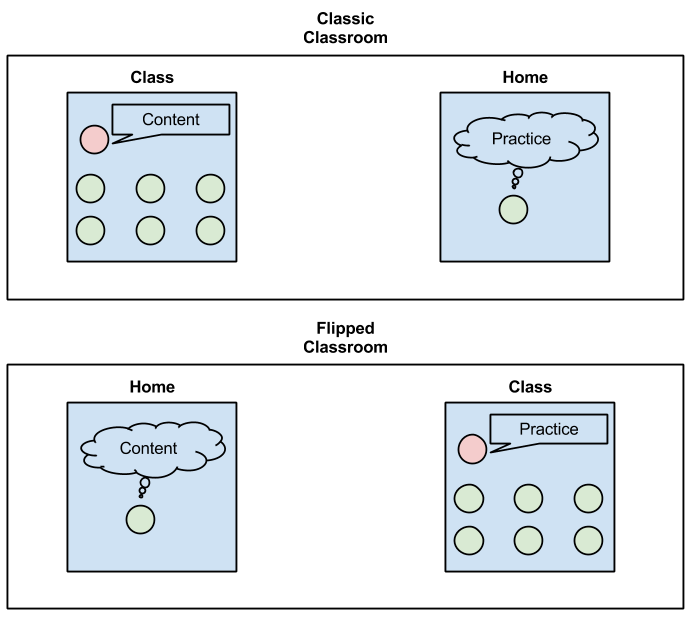
\includegraphics[width=.8\textwidth]{./static/flipped_class.png}
        \end{center}
    \end{frame}

    \begin{frame}
        \Huge
        \begin{center}
            Video
        \end{center}
    \end{frame}

    \begin{frame}
		\begin{center}
			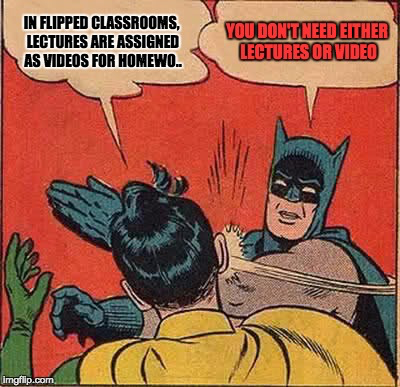
\includegraphics[width=.6\textwidth]{./static/time_for_this_again.png}
		\end{center}
	\end{frame}

    \begin{frame}
        \Huge
        \begin{center}
			Initial contact.
        \end{center}
    \end{frame}

    \begin{frame}
		\begin{center}
            \frame{
\includegraphics[height=.8\textheight]{./static/flipped_learning.jpg}}
		\end{center}
	\end{frame}

	\begin{frame}
		\begin{center}
			\Large
			Example 1: Final year game theory class
		\end{center}
	\end{frame}

    \begin{frame}
        \begin{center}
			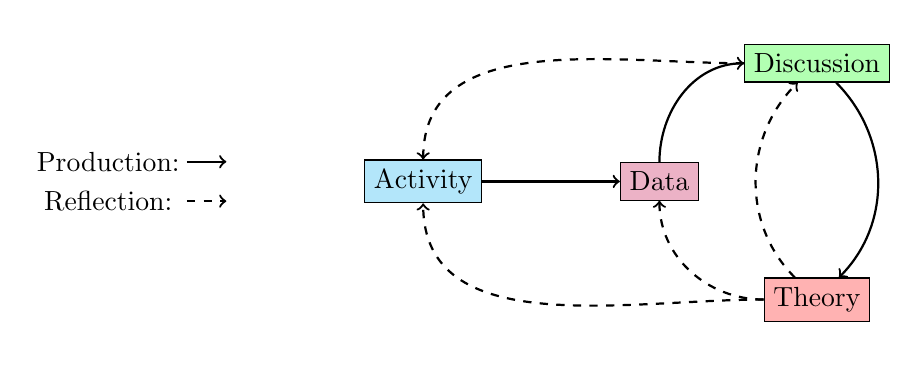
\begin{tikzpicture}
				% Nodes
				\node (activity) at (0,0) [fill=cyan!30, draw] {Activity};
				\node (data) at ($(activity) + (3,0)$) [fill=purple!30, draw] {Data};
				\node (discussion) at ($(data) + (2,1.5)$) [fill=green!30, draw] {Discussion};
				\node (theory) at ($(data) + (2,-1.5)$) [fill=red!30, draw] {Theory};

				% Creative arrows
				\draw [thick, ->] (activity) -- (data);
				\draw [thick, ->] (data) edge[out=90, in=180] (discussion);
				\draw [thick, ->] (discussion) edge[out=-45, in=45] (theory);

				% Reflective arrows
				\draw [thick, ->, dashed] (theory) edge[out=180, in=-90] (data);
				\draw [thick, ->, dashed] (theory) edge[out=180, in=-90] (activity);
				\draw [thick, ->, dashed] (discussion) edge[out=180, in=90] (activity);
				\draw [thick, ->, dashed] (theory) edge[out=135, in=-135] (discussion);

				% Key
				\draw [thick, ->] ($(activity) + (-3,.25)$) -- ($(activity) + (-2.5,.25)$);
				\node at ($(activity) + (-4, .25)$) {Production:};
				\draw [thick, ->, dashed] ($(activity) + (-3,-.25)$) -- ($(activity) +
				(-2.5,-.25)$);
				\node at ($(activity) + (-4, -.25)$) {Reflection:};

			\end{tikzpicture}
        \end{center}

        \begin{center}
            \textbf{Playing Games: A Case Study in Active Learning Applied to Game Theory} Knight. 2015 (MSOR Connections)
        \end{center}
	\end{frame}

    \begin{frame}
        \begin{center}
            \includegraphics[width=.8\textwidth]{./static/white_board.jpg}
        \end{center}
    \end{frame}

	\begin{frame}
		\begin{center}
			\Large
			Example 2: First year programming class
		\end{center}
	\end{frame}

    \begin{frame}
        \begin{center}
            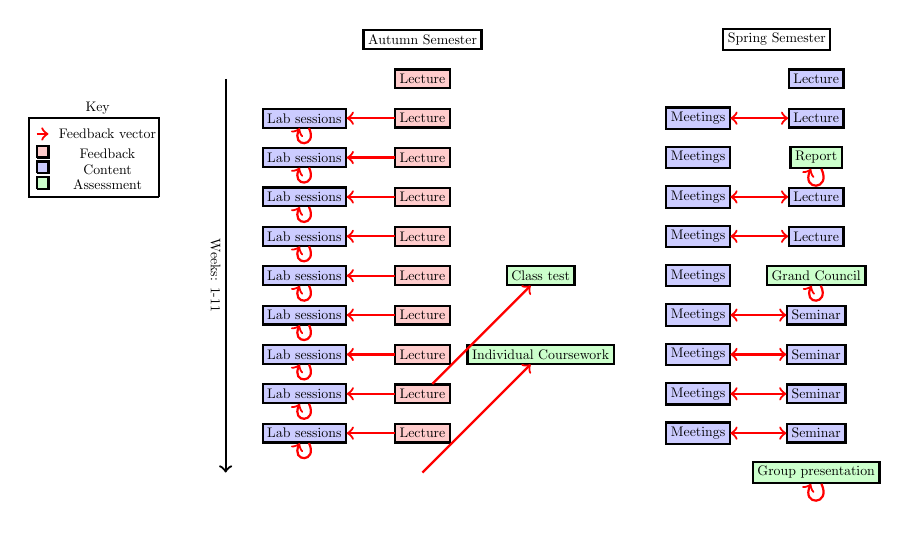
\begin{tikzpicture}[thick,scale=0.5, every node/.style={scale=0.5}]
\begin{scope}[xshift=-3cm, yshift=-3cm]
    \node at (-2.25, 3.25) {Key};
    % Color key
    \draw (-.7, 1) -- (-4, 1) -- (-4, 3) -- (-.7, 3) -- (-.7, 1);
    % Feedback
    \draw [fill=green!20] (-3.8, 1.2) -- (-3.8, 1.5) -- (-3.5, 1.5) -- (-3.5, 1.2) -- (-3.8, 1.2);
    \node at (-2, 1.3) {Assessment};
    % Content
    \draw [fill=blue!20] (-3.8, 1.6) -- (-3.8, 1.9) -- (-3.5, 1.9) -- (-3.5, 1.6) -- (-3.8, 1.6);
    \node at (-2, 1.7) {Content};
    % Assessment
    \draw [fill=red!20] (-3.8, 2) -- (-3.8, 2.3) -- (-3.5, 2.3) -- (-3.5, 2) -- (-3.8, 2);
    \node at (-2, 2.1) {Feedback};
    % Feedback direction
    \draw [red, ->] (-3.8, 2.6) -- (-3.5,2.6);
    \node  at (-2, 2.6) {Feedback vector};
\end{scope}
%------------ Weeks
\draw [->] (-2,1) -- (-2,-9) node [midway, below, rotate=-90] {Weeks: 1-11};


% ----------- Autumn
\node [rectangle, draw] at (3,2) {Autumn Semester};
% Draw lab session boxes
\node (week2) [rectangle, draw, fill=blue!20] at (0,0) {Lab sessions};
\node (week3) [rectangle, draw, fill=blue!20] at (0,-1) {Lab sessions};
\node (week4) [rectangle, draw, fill=blue!20] at (0,-2) {Lab sessions};
\node (week5) [rectangle, draw, fill=blue!20] at (0,-3) {Lab sessions};
\node (week6) [rectangle, draw, fill=blue!20] at (0,-4) {Lab sessions};
\node (week7) [rectangle, draw, fill=blue!20] at (0,-5) {Lab sessions};
\node (week8) [rectangle, draw, fill=blue!20] at (0,-6) {Lab sessions};
\node (week9) [rectangle, draw, fill=blue!20] at (0,-7) {Lab sessions};
\node (week10) [rectangle, draw, fill=blue!20] at (0,-8) {Lab sessions};
% Draw Lecture boxes
\node (lec1) [rectangle, draw, fill=red!20] at (3,1) {Lecture};
\node (lec2) [rectangle, draw, fill=red!20] at (3,0) {Lecture};
\node (lec3) [rectangle, draw, fill=red!20] at (3,-1) {Lecture};
\node (lec4) [rectangle, draw, fill=red!20] at (3,-2) {Lecture};
\node (lec5) [rectangle, draw, fill=red!20] at (3,-3) {Lecture};
\node (lec6) [rectangle, draw, fill=red!20] at (3,-4) {Lecture};
\node (lec7) [rectangle, draw, fill=red!20] at (3,-5) {Lecture};
\node (lec8) [rectangle, draw, fill=red!20] at (3,-6) {Lecture};
\node (lec9) [rectangle, draw, fill=red!20] at (3,-7) {Lecture};
\node (lec10) [rectangle, draw, fill=red!20] at (3,-8) {Lecture};
% Draw feedback arrows
\draw [red, ->] (lec2) -- (week2);
\draw [red, ->] (week2) to [out=-65, in=-115, looseness=6]  (week2);
\draw [red, ->] (lec3) -- (week3);
\draw [red, ->] (week3) to [out=-65, in=-115, looseness=6]  (week3);
\draw [red, ->] (lec4) -- (week4);
\draw [red, ->] (week4) to [out=-65, in=-115, looseness=6]  (week4);
\draw [red, ->] (lec5) -- (week5);
\draw [red, ->] (week5) to [out=-65, in=-115, looseness=6]  (week5);
\draw [red, ->] (lec6) -- (week6);
\draw [red, ->] (week6) to [out=-65, in=-115, looseness=6]  (week6);
\draw [red, ->] (lec7) -- (week7);
\draw [red, ->] (week7) to [out=-65, in=-115, looseness=6]  (week7);
\draw [red, ->] (lec8) -- (week8);
\draw [red, ->] (week8) to [out=-65, in=-115, looseness=6]  (week8);
\draw [red, ->] (lec9) -- (week9);
\draw [red, ->] (week9) to [out=-65, in=-115, looseness=6]  (week9);
\draw [red, ->] (lec10) -- (week10);
\draw [red, ->] (week10) to [out=-65, in=-115, looseness=6]  (week10);
% Highlight assessment
\node (ass1) [rectangle, draw, fill=green!20] at (6,-4) {Class test};
\node (ass2) [rectangle, draw, fill=green!20] at (6,-6) {Individual Coursework};
% Feedback loops for assessment
\draw [red, ->] (lec9) -- (ass1);
\draw [red, ->] (3, -9) -- (ass2);
% ----------- Spring
\begin{scope}[xshift=10cm]
\node [rectangle, draw] at (2,2) {Spring Semester};
% Draw lab session boxes
\node (week2) [rectangle, draw, fill=blue!20] at (0,0) {Meetings};
\node (week3) [rectangle, draw, fill=blue!20] at (0,-1) {Meetings};
\node (week4) [rectangle, draw, fill=blue!20] at (0,-2) {Meetings};
\node (week5) [rectangle, draw, fill=blue!20] at (0,-3) {Meetings};
\node (week6) [rectangle, draw, fill=blue!20] at (0,-4) {Meetings};
\node (week7) [rectangle, draw, fill=blue!20] at (0,-5) {Meetings};
\node (week8) [rectangle, draw, fill=blue!20] at (0,-6) {Meetings};
\node (week9) [rectangle, draw, fill=blue!20] at (0,-7) {Meetings};
\node (week10) [rectangle, draw, fill=blue!20] at (0,-8) {Meetings};
% Draw Lecture boxes
\node (lec1) [rectangle, draw, fill=blue!20] at (3,1) {Lecture};
\node (lec2) [rectangle, draw, fill=blue!20] at (3,0) {Lecture};
\node (lec3) [rectangle, draw, fill=green!20] at (3,-1) {Report};
\node (lec4) [rectangle, draw, fill=blue!20] at (3,-2) {Lecture};
\node (lec5) [rectangle, draw, fill=blue!20] at (3,-3) {Lecture};
\node (lec6) [rectangle, draw, fill=green!20] at (3,-4) {Grand Council};
\node (lec7) [rectangle, draw, fill=blue!20] at (3,-5) {Seminar};
\node (lec8) [rectangle, draw, fill=blue!20] at (3,-6) {Seminar};
\node (lec9) [rectangle, draw, fill=blue!20] at (3,-7) {Seminar};
\node (lec10) [rectangle, draw, fill=blue!20] at (3,-8) {Seminar};
\node (lec11) [rectangle, draw, fill=green!20] at (3,-9) {Group presentation};
% Draw feedback arrows
\draw [red, <->] (lec2) -- (week2);
\draw [red, <->] (lec4) -- (week4);
\draw [red, <->] (lec5) -- (week5);
\draw [red, <->] (lec7) -- (week7);
\draw [red, <->] (lec8) -- (week8);
\draw [red, <->] (lec9) -- (week9);
\draw [red, <->] (lec10) -- (week10);
% Highlight assessment
\draw [red, ->] (lec11) to [out=-65, in=-115, looseness=6] (lec11);
\draw [red, ->] (lec6) to [out=-65, in=-115, looseness=6] (lec6);
\draw [red, ->] (lec3) to [out=-65, in=-115, looseness=6] (lec3);
\end{scope}
\end{tikzpicture}
        \end{center}
    \end{frame}

    \begin{frame}
        \begin{center}
			\Large
            \textbf{FAQ:} Yes, great but [subject] is different.
        \end{center}
    \end{frame}

    \begin{frame}
        \begin{center}
			\Large
            \textbf{FAQ:} If I record my class will students no longer attend?
        \end{center}
    \end{frame}

	\begin{frame}
		\begin{center}
			\Large
			\textbf{FAQ:} If students don't [do some activity] before class what
            should I do?
		\end{center}
	\end{frame}

    \begin{frame}
        \begin{center}
			\Large
            \textbf{FAQ:} I have seen [a good talk] on flipped learning, isn't
            that ironic?
        \end{center}
    \end{frame}

	\begin{frame}
		\begin{center}
			\Large
			\textbf{FAQ:} I tried the flipped classroom and students don't like it.
		\end{center}
	\end{frame}

	\begin{frame}
		\begin{center}
			\Large
			\textbf{FAQ:} How much more work is it?
		\end{center}
	\end{frame}

    \begin{frame}
        \begin{center}
            \Large
            Reaction.
        \end{center}
    \end{frame}

    \begin{frame}
        \begin{center}
            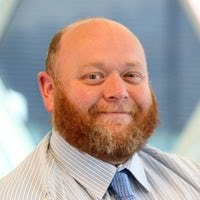
\includegraphics[width=.5\textwidth]{./static/Rutherford_Stephen_staff_profile.jpg}

            (Dr Stephen Rutherford. BIOSCI.)
        \end{center}
    \end{frame}

    \begin{frame}
        \begin{center}
            \normalsize
            Vince: \href{https://twitter.com/drvinceknight}{@drvinceknight}
            \texttt{knightva@cardiff.ac.uk}
        \end{center}
    \end{frame}

\end{document}
